\section{Datos tomados}

\newcolumntype{C}{>{$}c<{$}}
\begin{enumerate}
    \item Rendija de \qty{0.04}{\mm}
    

\setlength{\tabcolsep}{5pt}
\RenewDocumentCommand{\arraystretch}{}{1.2}
    \begin{tabular}{|C|C|}
        \hline
        \text{Intensidad} (\%)  & \text{Posición} (\si{\mm})\\
        \hline
        15.007019043    & -35.0096659775    \\
        15.4052734375   & -36.2796659525    \\
        16.5725708008   & -37.6343325925    \\
        19.1329956055   & -38.9889992325    \\
        22.4639892578   & -40.3436658725    \\
        25.0244140625   & -41.740665845     \\
        27.0874023438   & -43.0529991525    \\
        29.573059082    & -44.3229991275    \\
        33.0032348633   & -45.5929991025    \\
        38.0996704102   & -47.0323324075    \\
        43.9895629883   & -48.4716657125    \\
        47.3449707031   & -49.8263323525    \\
        \hline
    \end{tabular}
    \hspace{10pt}
    \begin{tabular}{|C|C|}
        \hline
        \text{Intensidad} (\%)  & \text{Posición} (\si{\mm})\\
        \hline
        46.2020874023   & -51.13866566      \\
        41.8273925781   & -52.4933323       \\
        36.3342285156   & -53.84799894      \\
        31.1645507812   & -55.20266558      \\
        26.6403198242   & -56.5996655525    \\
        23.0102539062   & -57.996665525     \\
        20.0286865234   & -59.3936654975    \\
        17.7917480469   & -60.79066547      \\
        16.2506103516   & -62.1876654425    \\
        15.4052734375   & -63.584665415     \\
        15.1062011719   & -65.02399872      \\
        \hline
    \end{tabular}

    $2Y_0 = \qty{30,0143327425}{\mm}$

    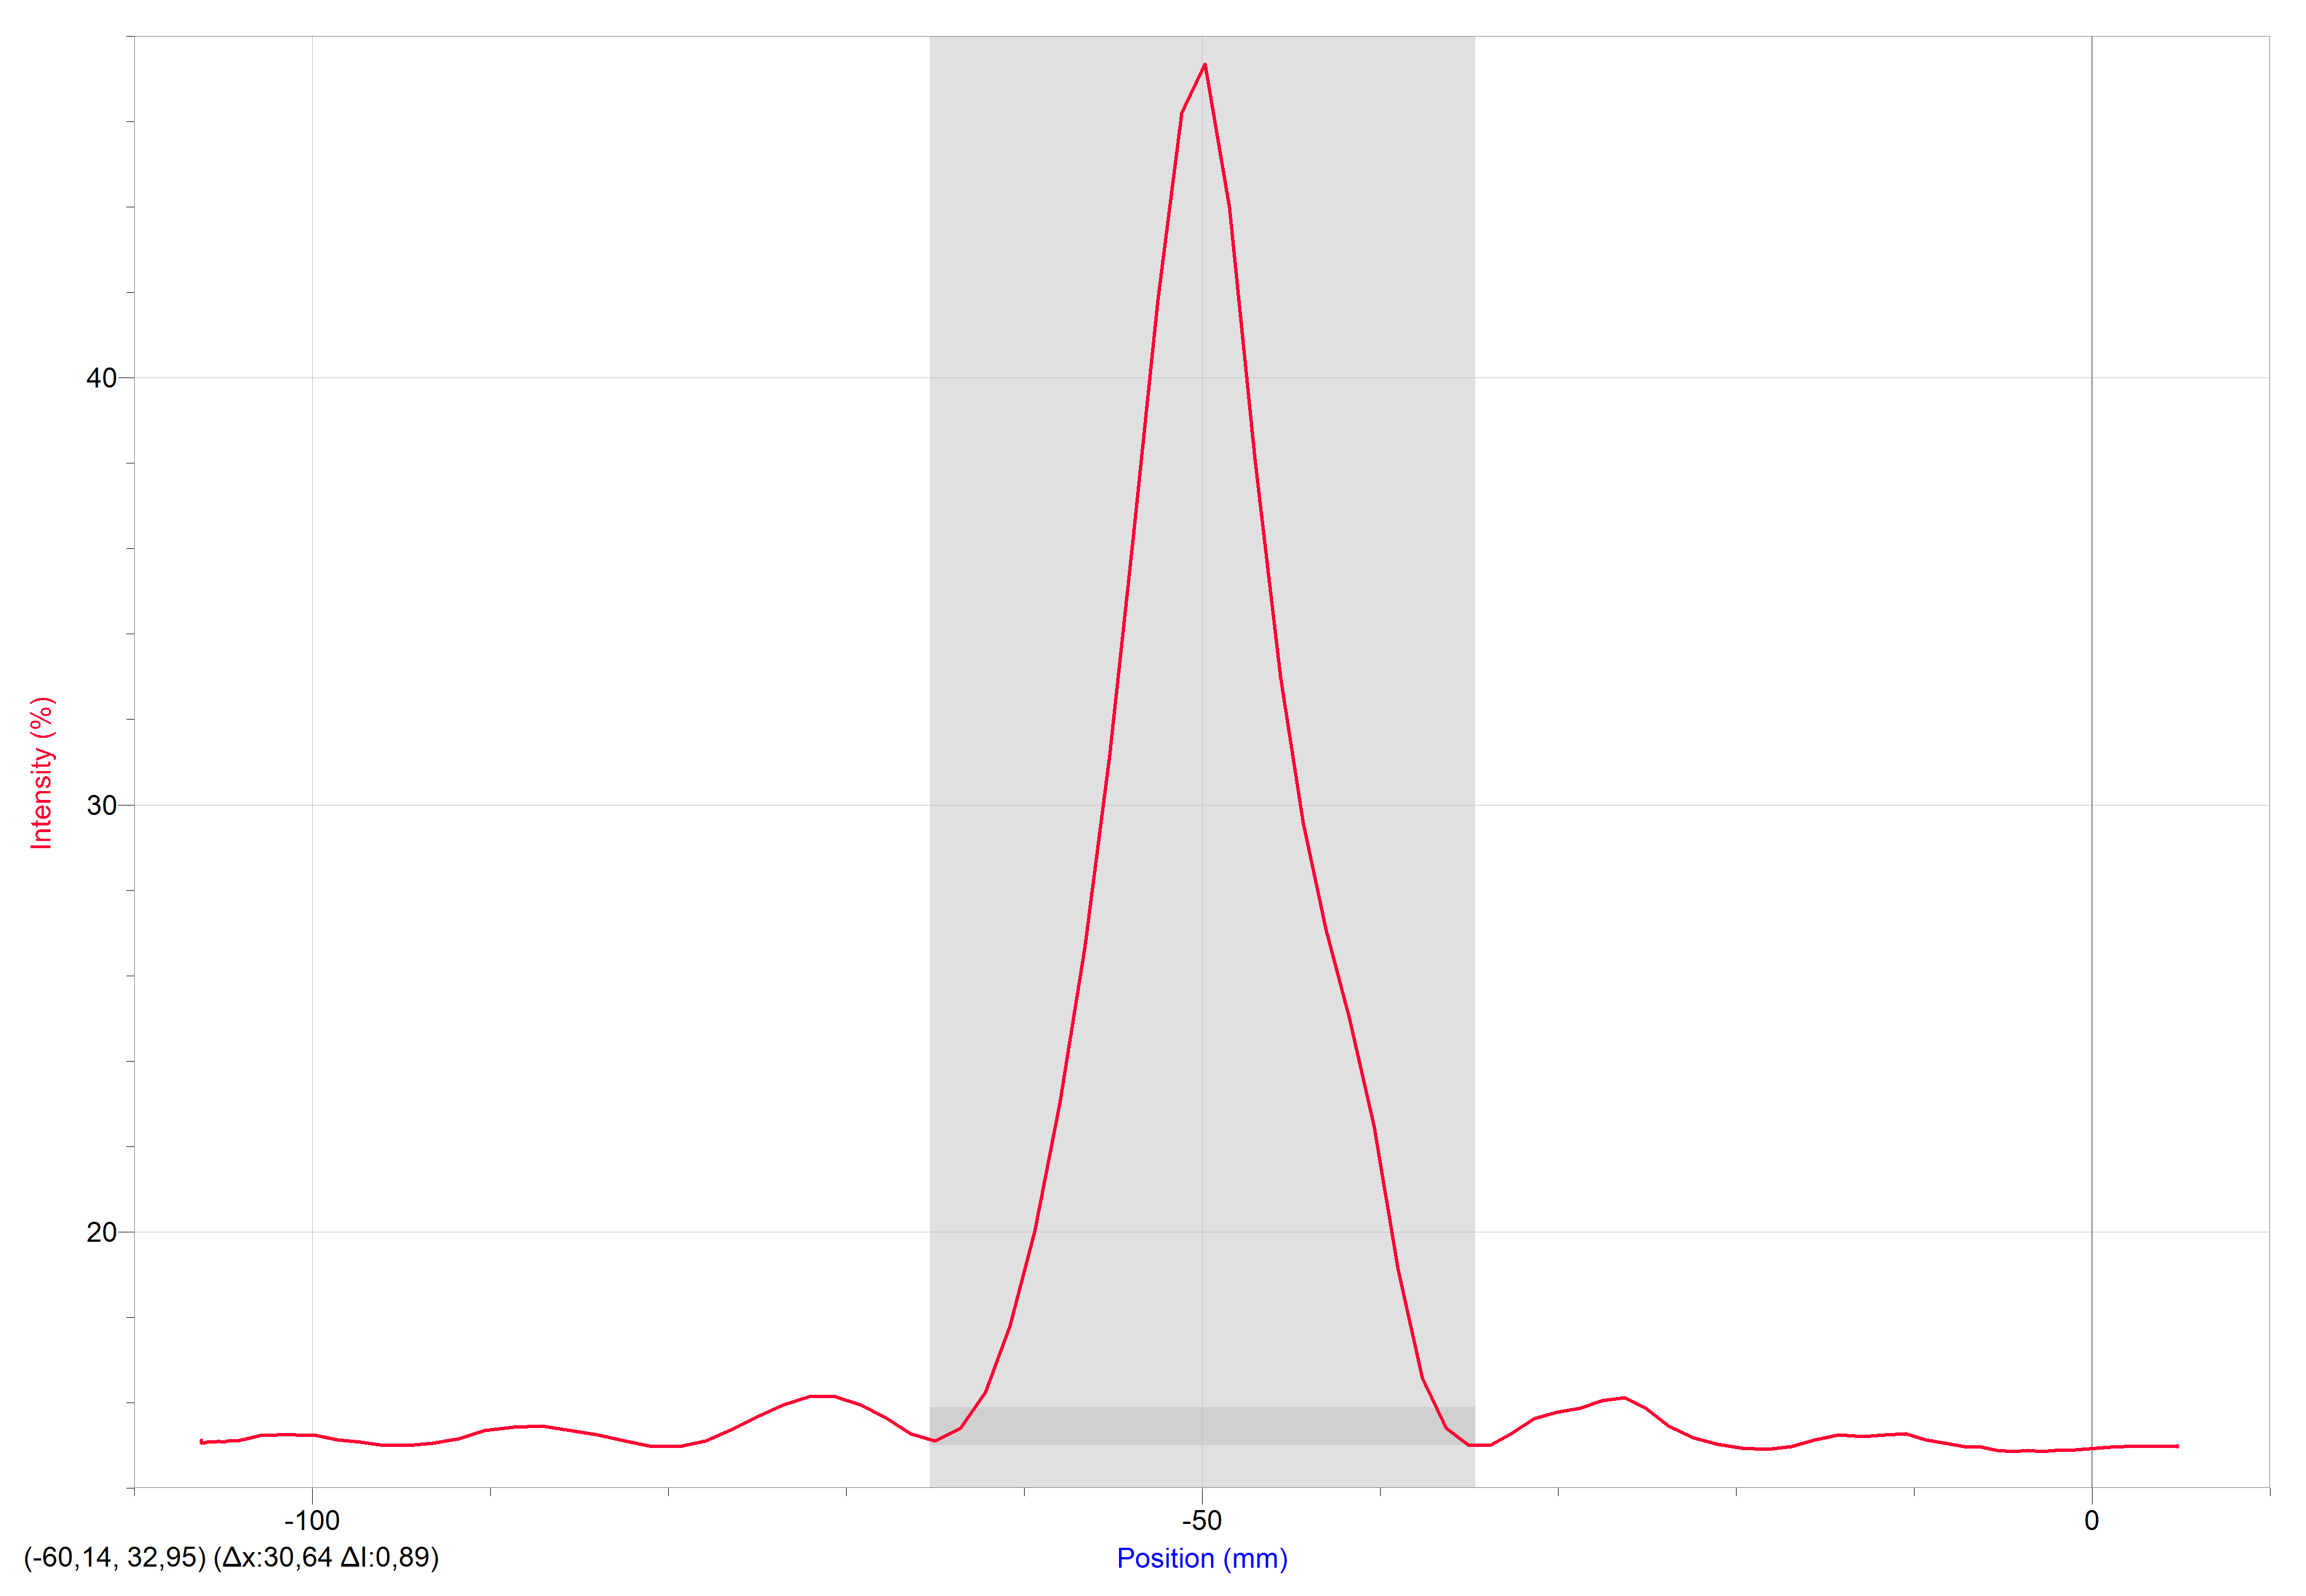
\includegraphics[width=0.94\textwidth]{RendijaAncha/DobleRendija004.png}
    \clearpage

    \item Rendija de \qty{0.08}{\mm}
    

    \begin{tabular}{|C|C|}
        \hline
        \text{Intensidad} (\%)    & \text{Posición} (\si{\mm})\\
        \hline
        15.7531738281      & -42.0369991725 \\
        17.3431396484      & -42.7143324925 \\
        21.9665527344      & -43.34933248   \\
        29.2495727539      & -43.941999135  \\
        39.192199707       & -44.53466579   \\
        50.7263183594      & -45.1696657775 \\
        62.956237793       & -45.804665765  \\
        75.8316040039      & -46.481999085  \\
        90.5715942383      & -47.159332405  \\
        99.9984741211      & -47.7943323925 \\
        99.9984741211      & -48.42933238   \\
        99.9984741211      & -49.021999035  \\
        99.9984741211      & -49.6569990225 \\
        99.9984741211      & -50.2496656775 \\
        \hline
    \end{tabular}
    \hspace{10pt}
    \begin{tabular}{|C|C|}
        \hline
        \text{Intensidad} (\%)    & \text{Posición} (\si{\mm})\\
        \hline
        99.9984741211      & -50.884665665  \\
        99.9984741211      & -51.47733232   \\
        99.9664306641      & -52.0276656425 \\
        84.407043457       & -52.5356656325 \\
        68.2495117188      & -53.085998955  \\
        52.3666381836      & -53.6363322775 \\
        38.4216308594      & -54.1866656    \\
        28.205871582       & -54.7369989225 \\
        21.8185424805      & -55.20266558   \\
        17.9901123047      & -55.625998905  \\
        16.0766601562      & -56.0916655625 \\
        15.5792236328      & -56.5149988875 \\
        \hline
    \end{tabular}

    $2 Y_0 = \qty{14.477999715}{\mm}$
    
    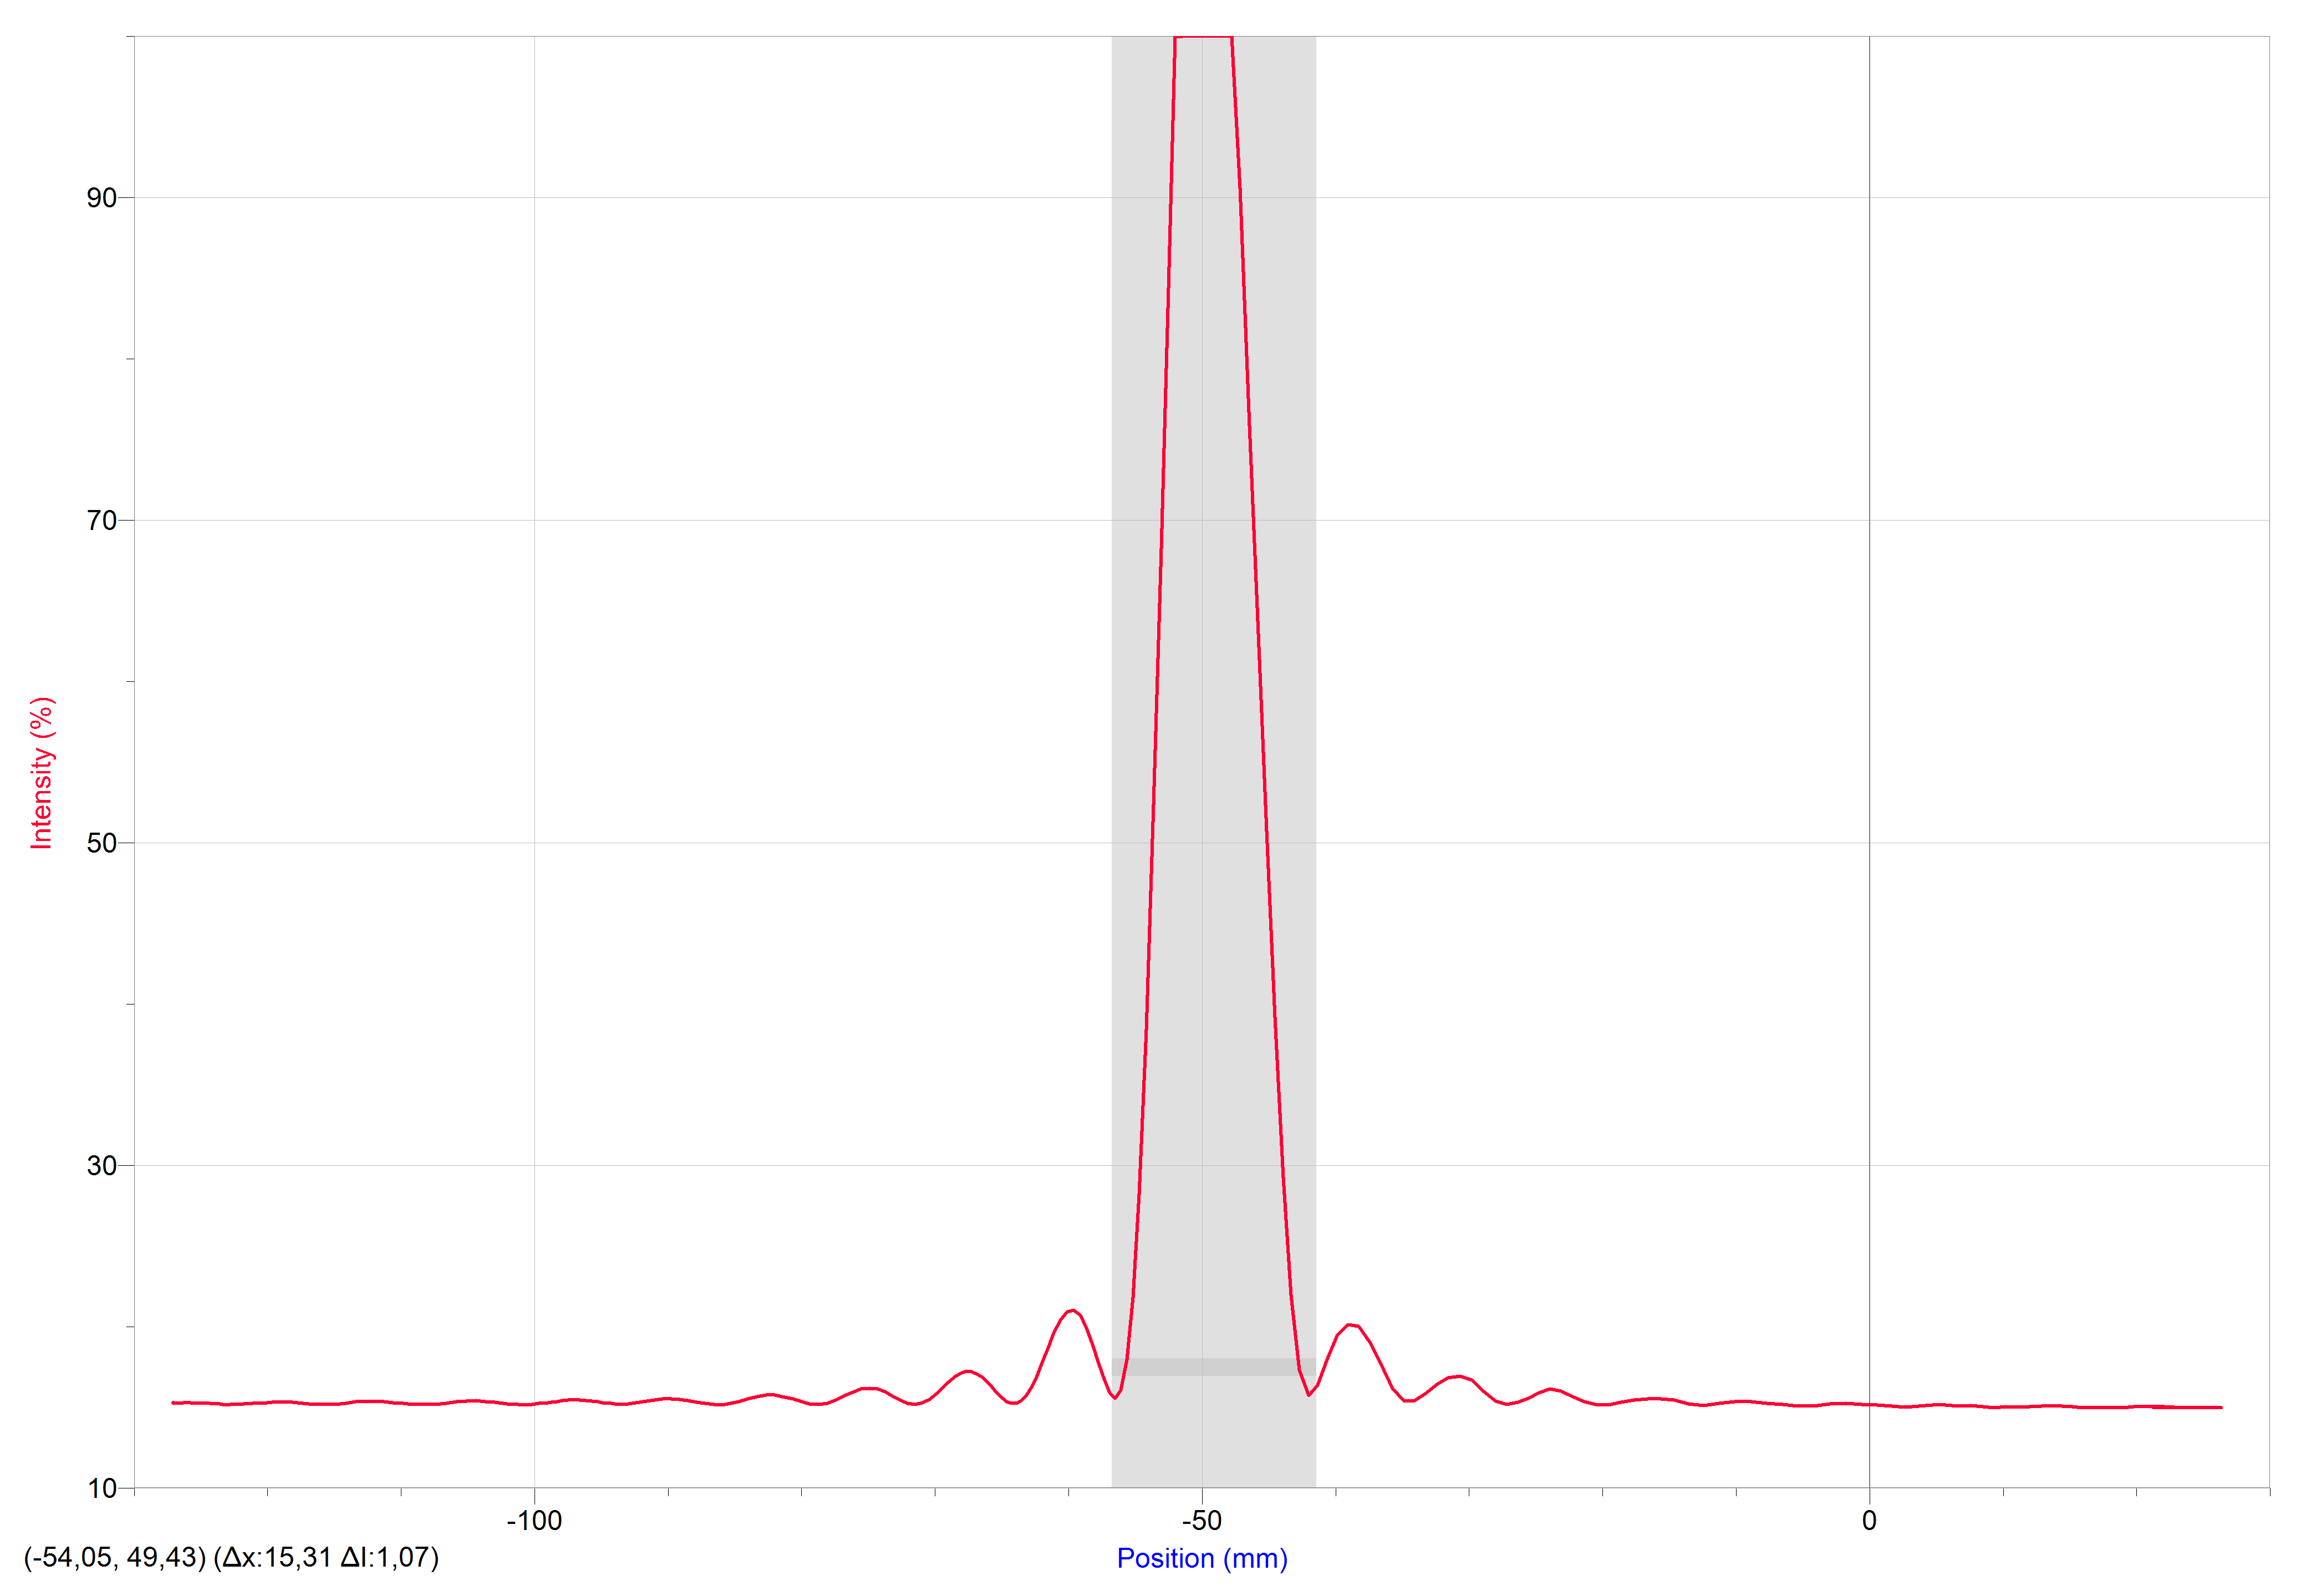
\includegraphics[width=0.94\textwidth]{RendijaAncha/DobleRendija008.png}
    % ~~~~ Aquí va imagen 0.08 ~~~~ %
    \clearpage
    \item Rendija de \qty{0.16}{\mm}
    
    \begin{tabular}{|C|C|}
        \hline
        \text{Intensidad} (\%)    & \text{Posición} (\si{\mm})\\
        \hline
        20.1278686523   & -45.465999105  \\
        34.5443725586   & -46.4396657525 \\
        99.9984741211   & -47.328665735  \\
        99.9984741211   & -48.1329990525 \\
        99.9984741211   & -48.8949990375 \\
        99.9984741211   & -49.5723323575 \\
        99.9984741211   & -50.2496656775 \\
        99.9984741211   & -50.884665665  \\
        99.9984741211   & -51.561998985  \\
        52.3910522461   & -52.2816656375 \\
        24.8748779297   & -52.9589989575 \\
        \hline
    \end{tabular}
    $2Y_0 = \qty{30,0143327425}{\mm}$

    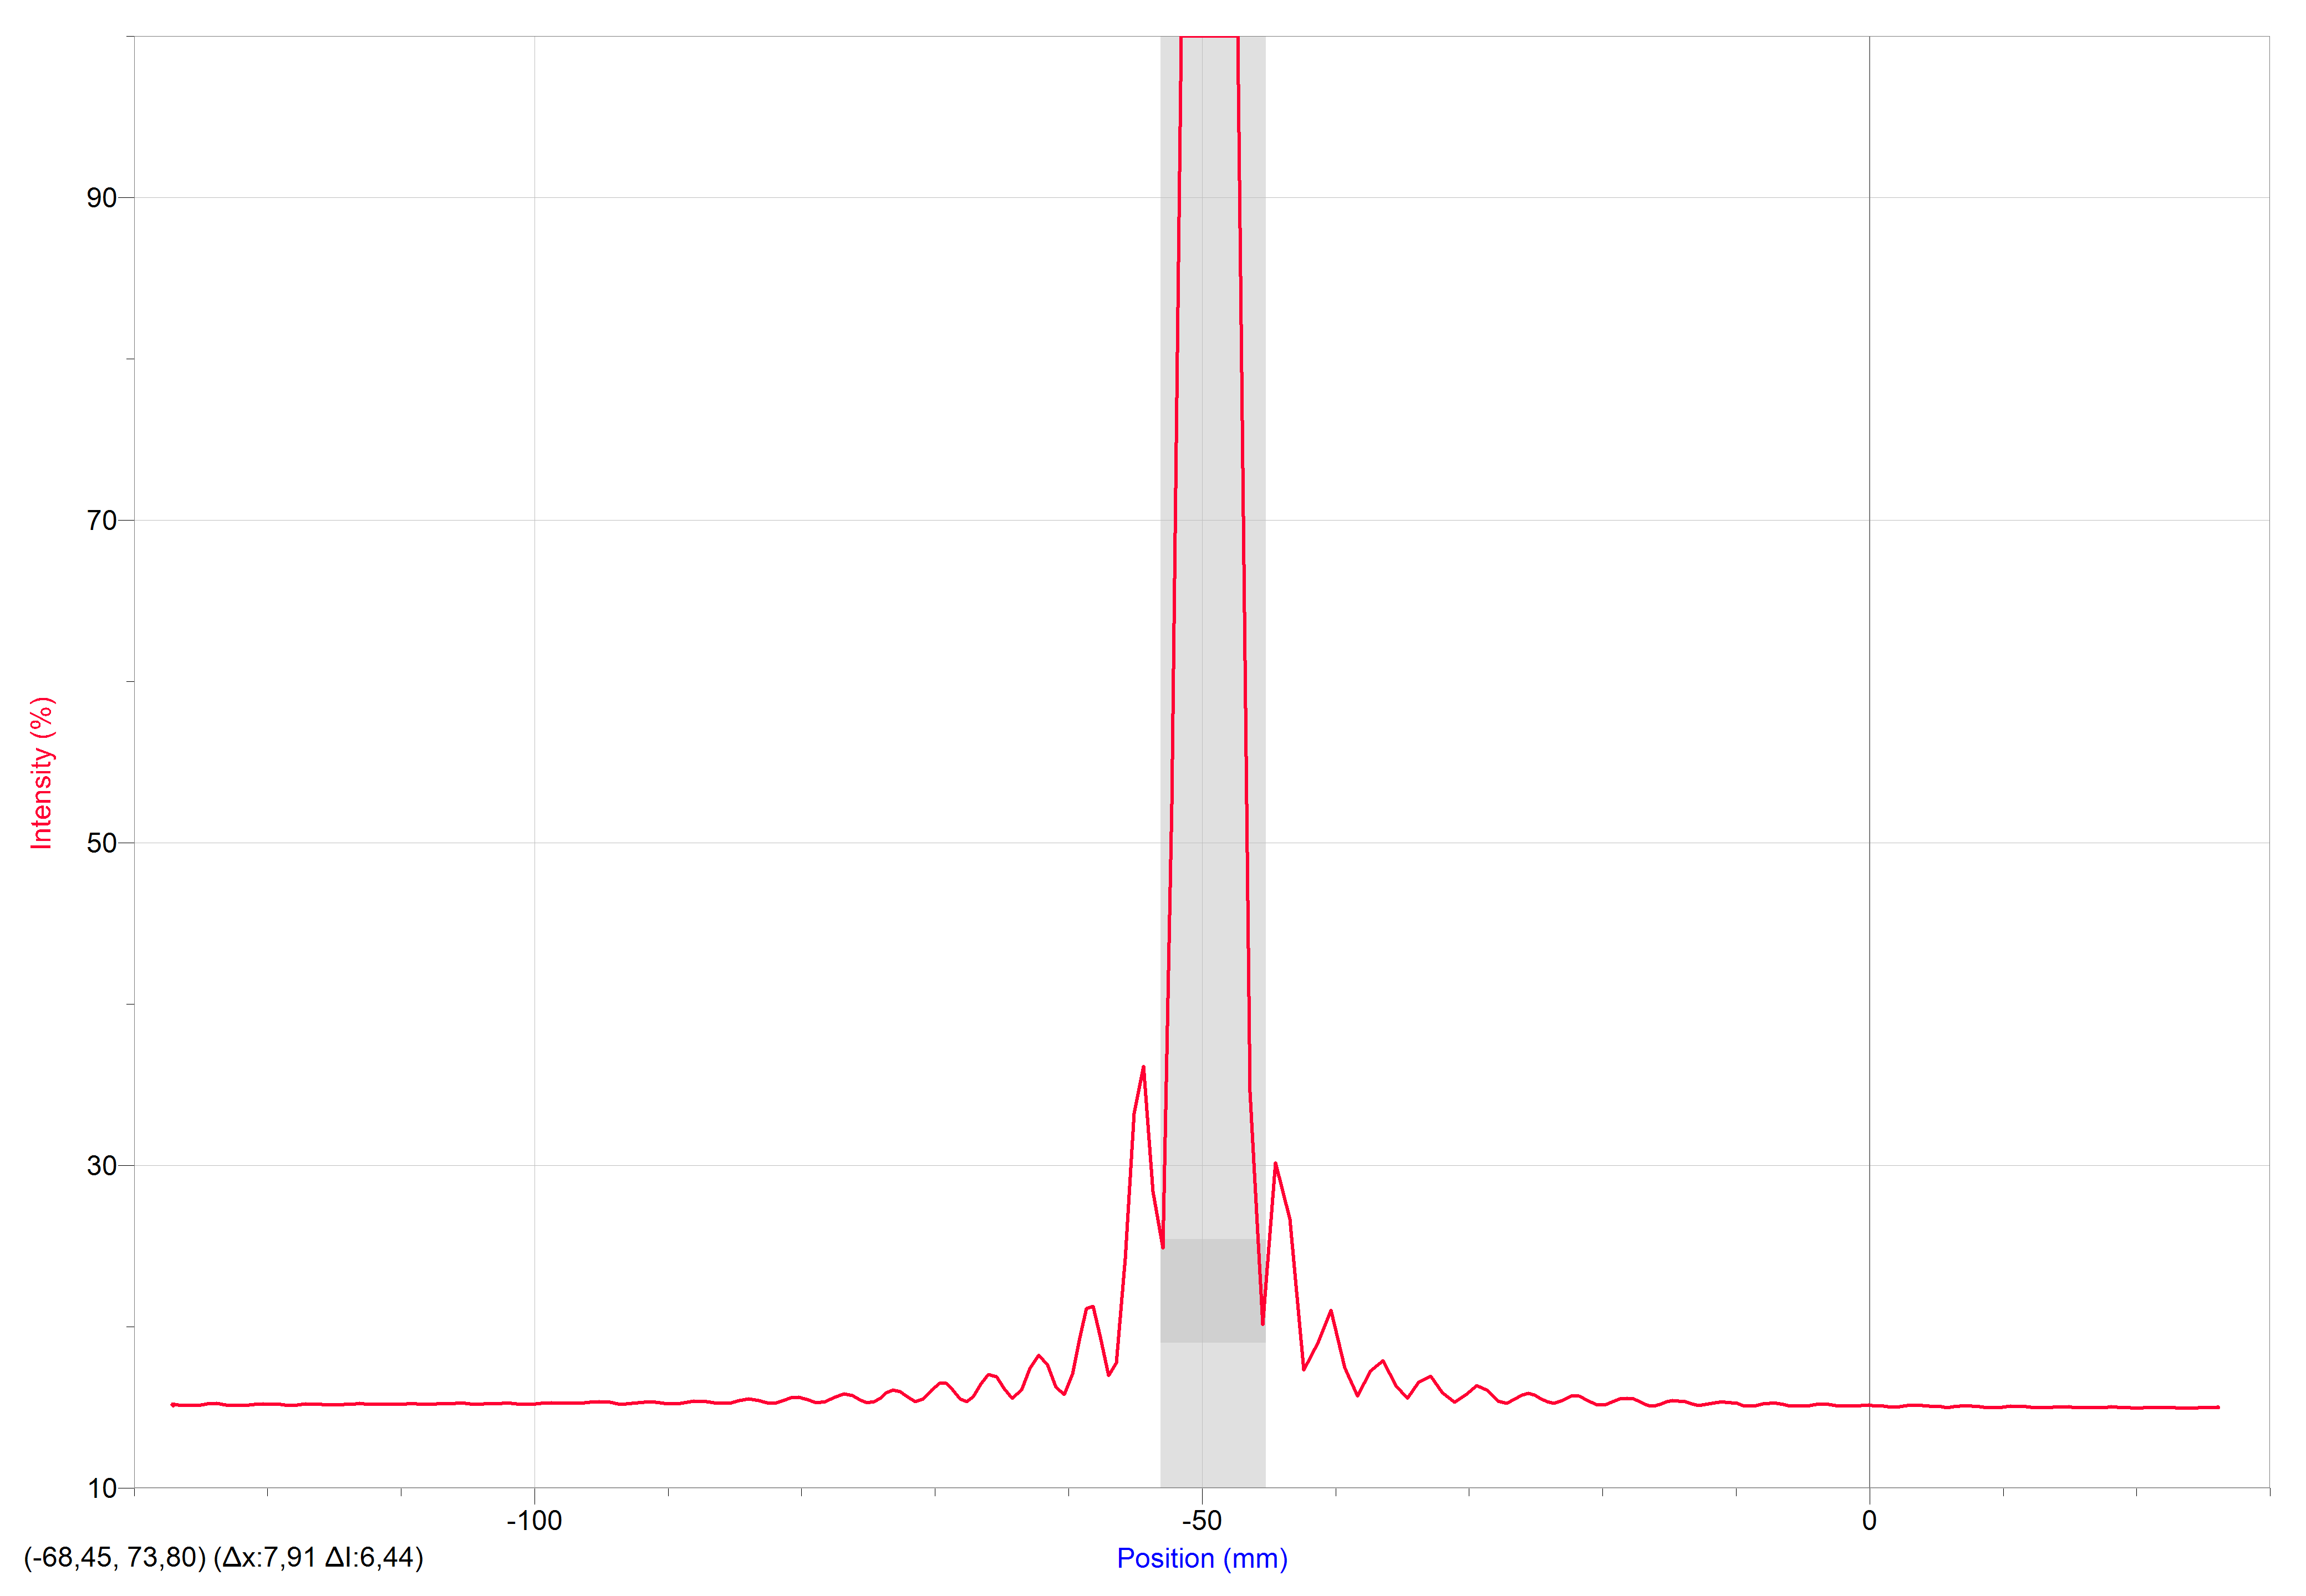
\includegraphics[width=0.94\textwidth]{RendijaAncha/RendijaAncha016.png}
    % ~~~~ Aquí va imagen 0.16 ~~~~ %
\end{enumerate}